\documentclass[12pt, a4paper, oneside]{article}
\usepackage{amsmath, amsthm, amssymb, appendix, bm, graphicx, hyperref, mathrsfs, cite,}

\title{\textbf{Homework 3: Segmentation}}

\author{Group 17 \\ Jiasheng Yun \quad 521030910093 \\ Zhan Su \quad 521030910112 \\ Shuwen Wu \quad 521030910087}

\author{
    \IEEEauthorblockN{Jiasheng Yun\textsuperscript{1}}
    \IEEEauthorblockA{\textit{521030910093}}
    \and
    \IEEEauthorblockN{Zhan Su\textsuperscript{2}}
    \IEEEauthorblockA{\textit{521030910112}}
    \and
    \IEEEauthorblockN{Shuwen Wu\textsuperscript{3}}
    \IEEEauthorblockA{\textit{521030910087}}
}


\date{\today}
\linespread{1.5}
\newtheorem{theorem}{定理}[section]
\newtheorem{definition}[theorem]{定义}
\newtheorem{lemma}[theorem]{引理}
\newtheorem{corollary}[theorem]{推论}
\newtheorem{example}[theorem]{例}
\newtheorem{proposition}[theorem]{命题}
\renewcommand{\abstractname}{\Large\textbf{摘要}}

\begin{document}

\maketitle

\setcounter{page}{0}
\maketitle
\thispagestyle{empty}

\begin{abstract}
    SAM\cite{2023arXiv230402643K} is a recent image segmentation model introduced by Meta that effectively identifies and separates objects within images. In this task, we fine-tune the model in specific areas of brain tumor segmentation of the MRI images.

\end{abstract}

\newpage
\pagenumbering{Roman}
\setcounter{page}{1}
\tableofcontents
\newpage
\setcounter{page}{1}
\pagenumbering{arabic}

\section{Introduction}

SAM is a recent image segmentation model introduced by Meta that effectively identifies and separates objects within images.  It is considered the first foundational model for Computer Vision.


The core idea behind the SAM model combines two techniques: image segmentation and self-supervised learning. It achieves this by first pretraining on self-supervised learning to learn a generic feature representation and then fine-tuning for specific tasks. During self-supervised pretraining, the model is trained on a large-scale dataset of unlabeled images to learn how to extract high-quality feature representations, thereby enhancing its generalization and robustness.

SAM’s architecture comprises three components that work together to return a valid segmentation mask:

1. An image encoder to generate one-time image embeddings.

2. A prompt encoder that embeds the prompts.

3. A lightweights mask decoder that combines the embeddings from the prompt and image encoders.

Image Encoder:  aims to map the image to be segmented into the image feature space.

Prompt Encoder: The prompt encoder encodes background points, masks, bounding boxes, or texts into an embedding vector in real time. The research considers two sets of prompts: sparse (points, boxes, text) and dense (masks). Points and boxes are represented by positional encodings and added with learned embeddings for each prompt type. Free-form text prompts are represented with an off-the-shelf text encoder from CLIP. Dense prompts, like masks, are embedded with convolutions and summed element-wise with the image embedding.

Mask Decoder: Integrate the two embeddings output by the image encoder and prompt encoder, and then decode the final segmentation mask from the feature map of these embeddings.
\begin{center}
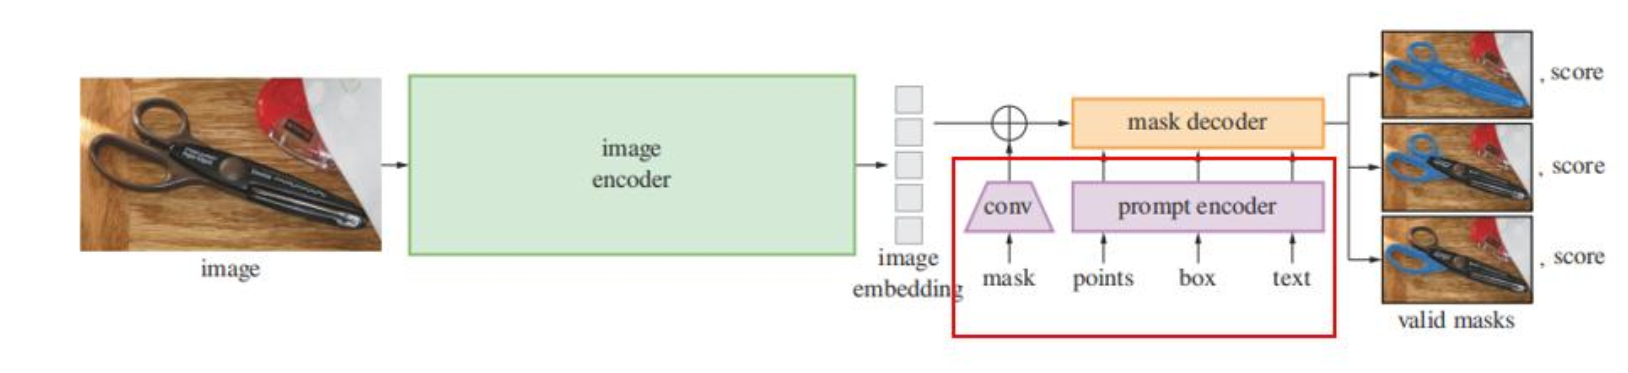
\includegraphics[width=1\textwidth]{1.png}
\caption{Fig1: The prompt encoder of SAM}
\end{center}
In SAM, the design and implementation of Prompt are key elements for the successful implementation of interactive segmentation tasks in the model. As a bridge between users and models, Prompt not only endows SAM with adaptability, but also endows users with the ability to guide the learning process of the model in a personalized way.

The design inspiration for SAM's Prompt comes from the need for interactive segmentation tasks. In this task, users need to guide the model in an intuitive and accurate way to focus on the areas of interest in the image. The introduction of Prompt enables SAM to achieve real-time interaction between users and models, thereby better meeting the requirements of specific segmentation tasks.

This is also why we can fine tune the model to apply it to specific areas of brain tumor segmentation of the MRI images. 

\section{Task-1: Box Prompt Training}
The SAM model underwent fine-tuning on a custom dataset, experimenting with different epochs, specifically 100, 200, and 400. After careful evaluation, we observed that there was no significant improvement in losses or IOU scores beyond the 100 epochs. Consequently, we determined that an epoch value of 100 would serve as our final result.

Subsequently, we conducted fine-tuning for the learning rate, exploring values such as 1e-2, 1e-3, 1e-4, 1e-5 1e-6 and 1e-7 and then calculated their average IOU as shown in Figure 2. Notably, when using a learning rate of 1e-2, the model struggled to converge, likely due to the excessively large learning rate, resulting in an average IOU of 0. For the remaining learning rates, the average IOU values were 0.4716, 0.6169, 0.6869, 0.6955 and 0.6883 respectively. For the remaining learning rates, we observed a steady improvement, with the best performance achieved at a learning rate of 1e-6.

\begin{center}
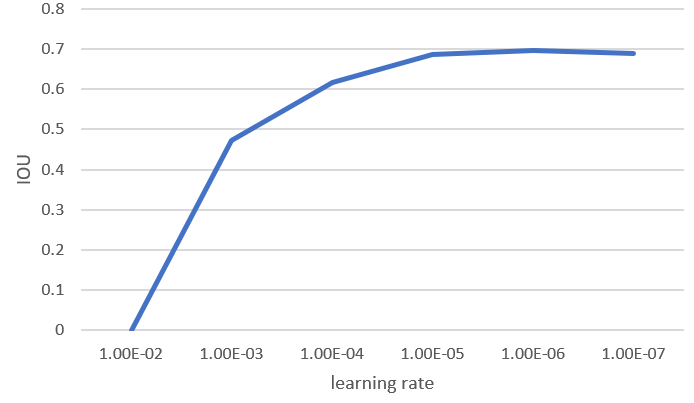
\includegraphics[width=1\textwidth]{4.png}
\caption{Fig2: Different learning rates and their corresponding IOUs}
\end{center}

To control the complexity of the model and mitigate overfitting, we introduced weight decay. However, the intriguing observation was that setting the learning rate to 1e-6 and weight decay to 1e-7 produced a final average IOU of 0.6954, almost identical to the result without weight decay. This finding suggests that the model's architecture is relatively simple, and the additional regularization from weight decay might not be necessary for our specific application.

Acknowledging the dynamic nature of training, we incorporated a learning rate scheduler into our regimen. The scheduler continuously adjusted the learning rate during the training process, enhancing model convergence and stability. This iterative adjustment played a crucial role in fine-tuning the SAM model, ensuring adaptability to the evolving training dynamics.

After extensive exploration of hyperparameters, we have come up with an optimized configuration that results in an IOU value of 0.7117 for the finely tuned sam partition. The final hyperparameters are as follows:

Learning Rate (lr): 2e-5

Weight Decay: 1e-7

Additionally, we implemented a learning rate scheduler to dynamically adjust the learning rate during training:
 
Learning Rate Scheduler: reduce the learning rate to half of its original size every ten steps.

In Figure 3, we visualize the evolution of the loss function throughout the training process.
\begin{center}
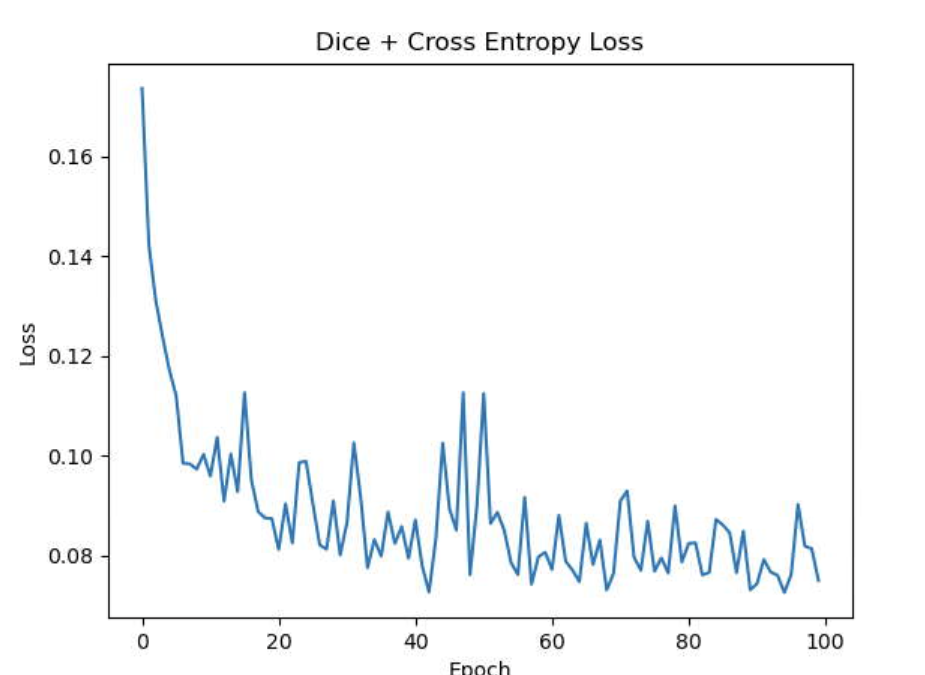
\includegraphics[width=1\textwidth]{2.png}
\caption{Fig3: Loss during the final model training process}
\end{center}

\section{Task-2: Points Prompt Training}
In this section, we prompt the model in points to make it applicable to specific areas of brain tumor segmentation of the MRI images. Compared to boxes, points are mainly used to mark specific locations of interest. Due to use point as guidance, the model's positioning accuracy is higher and can more accurately indicate the area of interest of the model. Therefore, if the task requires more precise positioning, especially for the segmentation of small or local targets, using Points is more appropriate. For the boxes, due to its coverage of a range, the model has a better tolerance for a certain degree of positional deviation, which allows users to guide the model more flexibly.

Similar to Boxes Prompt, we adjusted the hyperparameters of Points Prompt to achieve better training results. In the Points Prompt training, we also adjusted the Learning Rate and Weight Decay to find the optimal hyperparameter configuration.

We have attempted multiple learning rates, including 1e-2, 1e-3, 1e-4, 1e-5 and 1e-6 and calculated their average IOU as shown in Figure 4. Similar to Boxes Prompt, we found that when the learning rate is 1e-2, the model is difficult to converge, resulting in an average IOU of 0.0281. On the other learning rates, the average IOU values are 0.4601, 0.5600, 0.5653, and 0.5187. Obtain maximum value at a learning rate of 1e-5.

\begin{center}
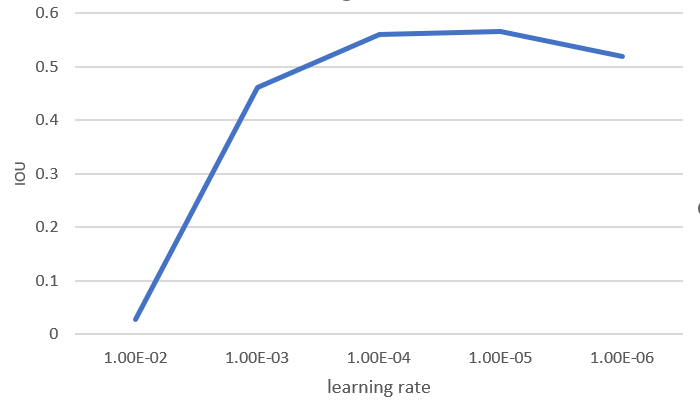
\includegraphics[width=1\textwidth]{3.png}
\caption{Fig4: Different learning rates and their corresponding IOUs}
\end{center}

In the process of fine-tuning the Points Prompt, we, like in the Boxes Prompt training, encountered challenges related to hyperparameter tuning, specifically in adjusting the Learning Rate and Weight Decay. Notably, during experimentation with different configurations, an interesting observation was made: the introduction of Weight Decay led to a decrease in Intersection over Union (IOU) values.

In the process of fine-tuning, we also adjusted the weight decay, just like the box prompt training. It is worth noting that in the experimental process of different configurations, we found that introducing weight decay resulted in a decrease in IOU values.

When Weight Decay was applied to the Points Prompt training, the IOU values exhibited a downward trend, contrary to our expected outcome. This unexpected behavior suggests that, for the this points prompt task, the regularization induced by Weight Decay might have inadvertently hindered the model's ability to capture intricate details or nuances associated with point-based guidance.

Afterwards, we attempted to introduce a learning rate scheduler, hoping to improve the performance of the model by dynamically adjusting the learning rate. Unfortunately, the scheduler also did not make the results more optimized.

After multiple experiments and adjustments on the Points Prompt, we ultimately chose a configuration with a learning rate of 1e-5. Under this configuration, we observed a relatively high average IOU value, indicating that the learning rate setting is more appropriate for specific brain tumor segmentation tasks.

\begin{center}
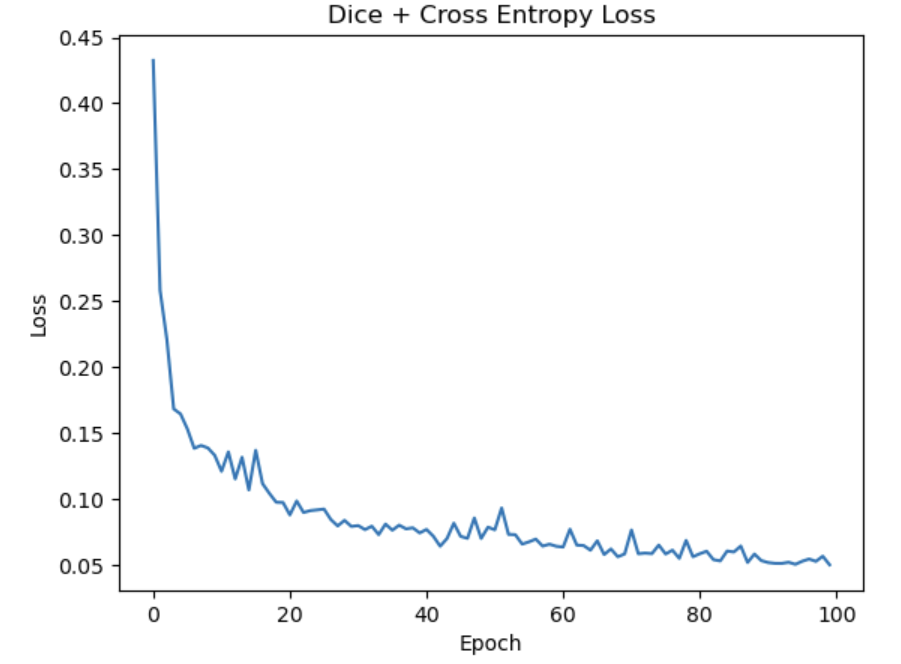
\includegraphics[width=1\textwidth]{6.png}
\caption{Fig5: Loss during the final model training process(points prompt)}
\end{center}

\begin{center}
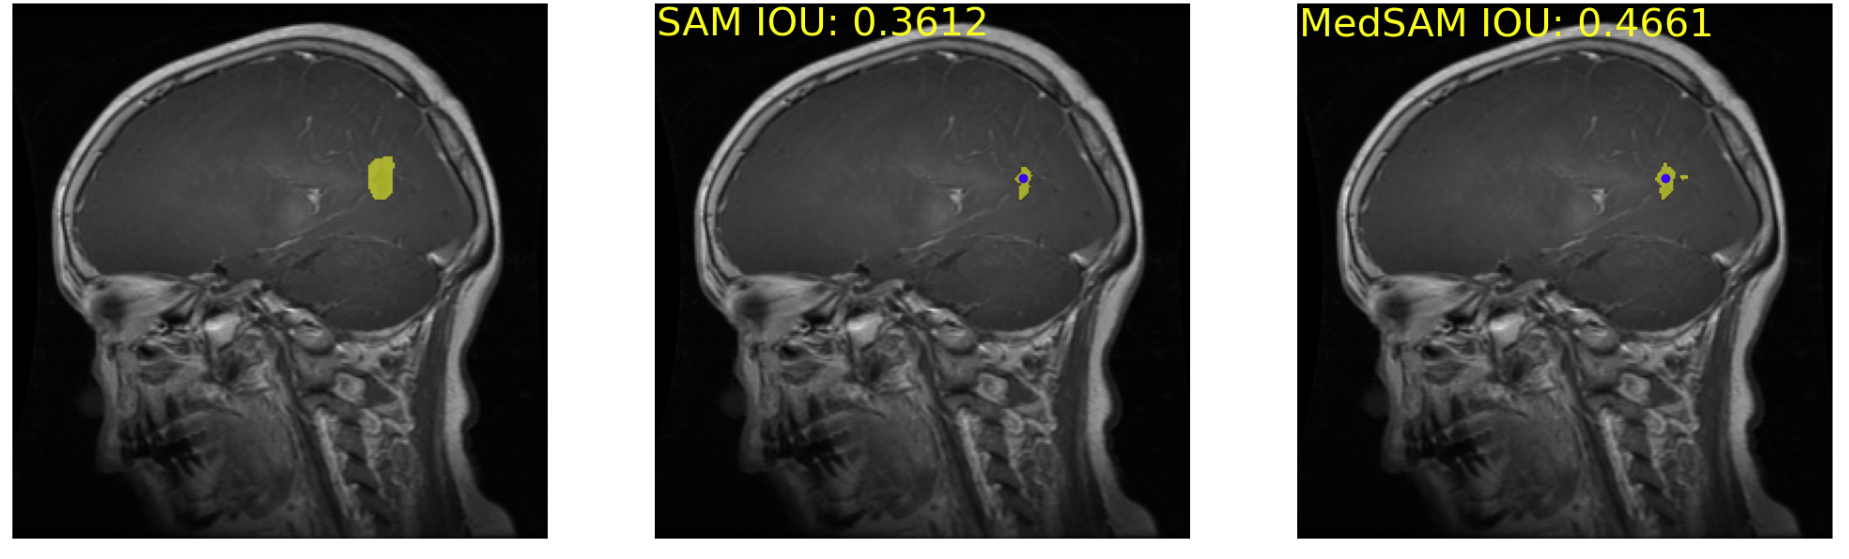
\includegraphics[width=1\textwidth]{5.png}
\caption{Fig6: Point Model testing sample}
\end{center}

\section{Summarize}
In this study, we conducted in-depth fine-tuning on the SAM model to make it suitable for specific brain tumor segmentation tasks. By conducting detailed experiments and adjustments on the training processes of two different Prompts, we have drawn a series of key conclusions and lessons learned.

Firstly, we found that an appropriate learning rate is key to achieving good performance in the training of Box Prompt and Points Prompt. A learning rate that is too high may make it difficult for the model to converge, while a learning rate that is too small may trap the model in local optima.

Secondly, we noticed that the introduction of Weight Decay in Points Prompt training resulted in an unexpected decrease in IOU values. This suggests that we need to be more cautious when using Weight Decay in specific tasks to avoid over regularization affecting the performance of the model.

Finally, we attempt to introduce a learning rate scheduler, hoping to improve model performance by dynamically adjusting the learning rate during the training process. However, it is effective in Box Prompt training but doesn't work in Points Prompt training. And this difference may be attributed to the characteristics of the task itself and the sensitivity of the model to different tasks. One of the reasons why the learning rate scheduler may be more effective in Box Prompt training is that the task involves segmenting relatively large regions. In this case, by dynamically adjusting the learning rate, the model can better adapt to different feature scales and complexities, which helps to improve the convergence and generalization performance of the model.
\newpage


\bibliography{1}
\bibliographystyle{plain}

\end{document}